\begin{example}[Nested Loop with Related Iterator]
  \label{ex:relatedNestedWhileSim}
  %
  %
  { \small
\begin{figure}
\centering
\begin{subfigure}{.4\textwidth}
  \begin{centering}
  {\small
  $
  \begin{array}{l}
      \kw{relatedNestedWhileSim}(n, N) \triangleq \\
      \clabel{ \assign{i}{n} }^{0} ; \\
          \ewhile ~ \clabel{i > 0}^{1} ~ \edo ~ \\
          \qquad \Big(
            \clabel{\assign{k}{i - N}}^{2};\\
            \qquad \ewhile ~ \clabel{k > 0}^{3} ~ \edo ~
            \Big(
              \clabel{\assign{k}{k - 1}}^{4}
                \Big); \\
                \qquad \clabel{\assign{i}{k + N}}^{5};
                \clabel{\assign{i}{i-1}}^{6}
            \Big)
      \end{array}
  $
  }
  \caption{}
  \end{centering}
  \end{subfigure}
\begin{subfigure}{.5\textwidth}
  \begin{centering}
%   \todo{abstract-cfg for two round}
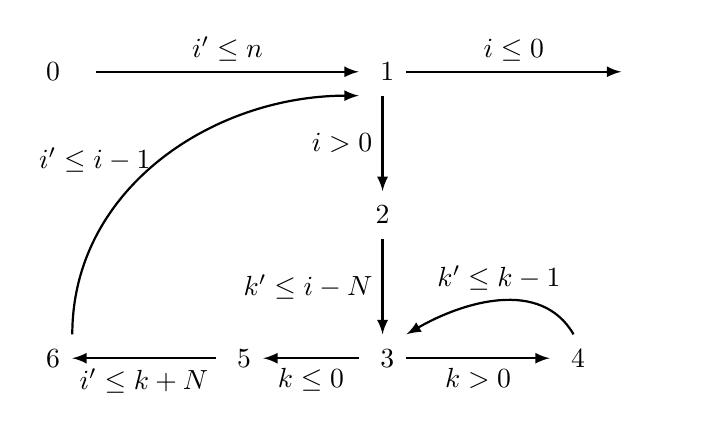
\begin{tikzpicture}[scale=\textwidth/20cm,samples=200]
\draw[] (-7, 10) circle (0pt) node{{ $0$}};
\draw[] (0, 10) circle (0pt) node{{ $1$}};
\draw[] (6, 10) circle (0pt) node {{$\lex$}};
\draw[] (0, 7) circle (0pt) node{{$2$}};
\draw[] (0, 4) circle (0pt) node{{ $3$}};
\draw[] (-7, 4) circle (0pt) node{{ $6$}};
\draw[] (-3, 4) circle (0pt) node{{ $5$}};
\draw[] (4, 4) circle (0pt) node{{ $4$}};
% Counter Variables
%
% Control Flow Edges:
\draw[ thick, -latex] (-6, 10)  -- node [above] {$i' \leq n$}(-0.5, 10);
\draw[ thick, -latex] (0, 9.5)  -- node [left] {$i > 0$} (0, 7.5) ;
\draw[ thick, -latex] (0, 6.5)  -- node [left] {$k' \leq i - N$} (0, 4.5) ;
\draw[ thick, -latex] (-0.5, 4)  -- node [below] {$k \leq 0$} (-2.5, 4) ;
\draw[ thick, -latex] (-3.5, 4)  -- node [below] {$i' \leq k + N$} (-6.5, 4) ;
\draw[ thick, -latex] (-6.5, 4.5)  to  [out=90,in=180]  node [left] {$i' \leq i - 1$ }(-0.5, 9.5);
\draw[ thick, -latex] (0.5, 10)  -- node [above] {$i \leq 0 $}  (5, 10);
\draw[ thick, -latex] (4, 4.5)  to  [out=120,in=30] node [above] {$k' \leq k - 1$}  (0.5, 4.5);
\draw[ thick, -latex] (0.5, 4)  -- node [below] {$k > 0$}  (3.5, 4);
\end{tikzpicture}
\caption{}
  \end{centering}
  \end{subfigure}
\caption{
(a) The Simplified Example of Nested Loop with Related Iterator
  (b) The Abstract Execution Control Flow Graph}
    \label{fig:relatedNestedWhileSim}
\end{figure}
}
\end{example}

\begin{enumerate}
  \item  \textbf{Abstract Control Flow Graph} is generated in Figure~\ref{fig:relatedNestedWhileSim}(b).

  \item \textbf{Program Refinement}
  \\
  The loop free simple transition paths:
  \[
      % \begin{array}{lllll}
          \tpath_0 = (0 \to 1)
          \quad
          \tpath_1 = (1 \to 2 \to 3)
          \quad           
          \tpath_2 = (3 \to 4 \to 3)
          \quad
          \tpath_3 = (3 \to 5 \to 6 \to 1)
          \quad
          \tpath_4 = (1 \to \lex)
      % \end{array}
      \]
  \textbf{Refined Program}:
  \[
  \rprog = \tpath_0 ; 1: \rprepeat(\tpath_1; 3: \rprepeat(\tpath_2); \tpath_3); \tpath_4
  \]
  %
 Let $\rprog_1 = \rprepeat(\tpath_1; 3: \rprepeat(\tpath_2); \tpath_3)$
\item {Path Local Reachability-bound}:
\\
$\outinB(\rprog, \tpath_0) = 1$ \quad
$\outinB(\rprog, \tpath_4) = 1$ \\
$\outinB(1: \rprog_1, \tpath_1) = N$ \\
$\outinB(1: \rprog_1, \tpath_3) = N$ \\
$\outinB(3: \rprepeat(\tpath_2), \tpath_2) = n - N$ 
\\
Loop Bounds:
\\
$BD(\tpath_0) = 1$
\quad
$BD(\tpath_4) = 1$
\quad
$BD(\rprepeat(\tpath_2)) = n - N $
\\
$BD(\rprepeat(\tpath_1; 3: \rprepeat(\tpath_2); \tpath_3)) = N $
%
\item Loop Reachability-bound:
\\
\highlight{
% $\lpchB(1: \rprog_1, \tpath_0) = 0$ \quad
$\lpchB(1: \rprog_1, \tpath_1) = N$ \quad
$\lpchB(1: \rprog_1, \tpath_3) = N$ \quad \\
\highlight{$\lpchB(1: \rprog_1, \tpath_2) = 1$} \quad
$\lpchB(3: \rprepeat(\tpath_2), \tpath_2) = n - N$ \quad
}
%
%
\item Path Global Reachability-bound:
\\
$\inoutB(\rprog, \tpath_0) = 1$ \quad
$\inoutB(\rprog, \tpath_1) = N$ \quad
$\inoutB(\rprog, \tpath_2) = 1 \times (n - N)$ \\
$\inoutB(\rprog, \tpath_3) = N$ \quad
$\inoutB(\rprog, \tpath_4) = 1$
%
\item The Reachability-bound:
\\
$\psRB(0) = \psRB(\lex) = 1$ \quad
$\psRB(1) = N + 1$ \quad
$\psRB(4) = n - N$ \quad \\
$\psRB(2) = \psRB(5) =  \psRB(6) = N$ \quad
\highlight{$\psRB(\{3\}) = N + n - N = n$}
\end{enumerate}